\documentclass[../../syllabus_1.tex]{subfiles}
\begin{document}

\chapter{Fractions et nombres décimaux}
 
\section*{Matières}
\begin{enumerate}[label=\textbf{\arabic*.}]
    \item Représentation d'une fraction.
    \item Fractions équivalentes.
    \item Inverse d'un nombre.
    \item Simplification et fractions irréductibles.
    \item Addition et soustraction de fractions de même dénominateur.
    \item Placement sur une droite graduée.
\end{enumerate}
 
\section{Á la découverte des fractions égyptiennes}
 
Dans l'Égypte antique (il y a plus de $4\,000$ ans), les scribes utilisaient un système numérique fascinant. Pour représenter des parts, ils n'utilisaient que des fractions unitaires (dont le numérateur est toujours $1$), à l'exception notable de $\frac{2}{3}$.
 
Ainsi, pour partager $5$ pains entre $6$ personnes, ils n'écrivaient pas $\frac{5}{6}$ comme nous, mais ils cherchaient une décomposition sous forme de somme de fractions différentes :
\begin{equation*}
    \frac{5}{6} = \frac{1}{2} + \frac{1}{3}
\end{equation*}
Cela signifiait concrètement : on donne d'abord un demi-pain à chacun ($\frac{1}{2} \times 6 = 3$ pains utilisés), puis un tiers de pain à chacun ($\frac{1}{3} \times 6 = 2$ pains utilisés). Le compte est bon !
 
\newpage
\section{Vocabulaire et représentation}
 
Une fraction représente un partage équitable (en parts parfaitement égales) d'une grandeur ou d'une unité.
 
Une écriture fractionnaire se présente sous la forme :
\begin{equation*}
    \dfrac{a \ (\text{Numérateur})}{b \ (\text{Dénominateur})}
\end{equation*}
où $a$ et $b$ sont des nombres entiers, avec $b \neq 0$ (car la division par zéro est impossible).
 
\begin{center}
    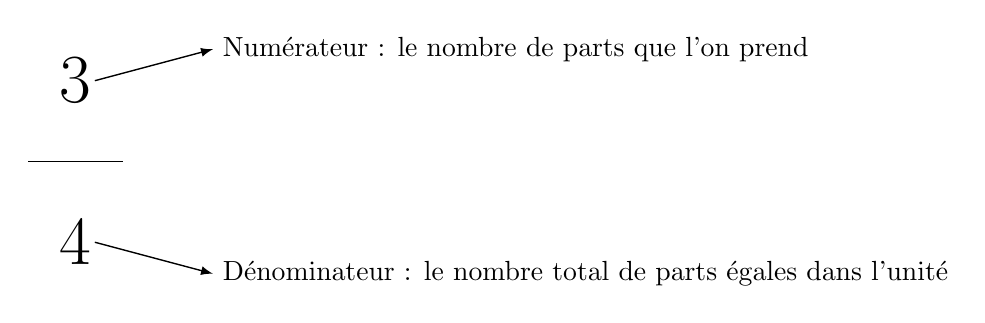
\begin{tikzpicture}[>=latex, line width=0.5pt]
        \begin{Huge}
            \draw (0,0)node[inner sep=1pt, anchor=south,name=N]{\(3\)};
            \draw (0,-1.4)node[inner sep=1pt, anchor=north,name=D]{\(4\)};
            \draw (-0.6,-0.7) -- (0.6,-0.7);
        \end{Huge}
        \draw[->] (N.east) --++(1.5,0.4) node[right, font=\normalsize]{Numérateur : le nombre de parts que l'on prend};
        \draw[->] (D.east) --++(1.5,-0.4) node[right, font=\normalsize]{Dénominateur : le nombre total de parts égales dans l'unité};
    \end{tikzpicture}
\end{center}
 
\begin{itemize}
    \item Le \textbf{numérateur} (en haut) indique le nombre de parts que l'on prend ou que l'on considère.
    \item Le \textbf{dénominateur} (en bas) indique en combien de parts égales l'unité a été partagée.
    \item La \textbf{barre de fraction} symbolise l'opération de division.
\end{itemize}
 
Par exemple, prenons une tablette de chocolat rectangulaire de $12$ carrés. Si Sarah mange $\frac{3}{4}$ de la tablette :
\begin{itemize}
    \item le dénominateur ($4$) indique qu'on doit couper la tablette en $4$ blocs égaux (chaque bloc contiendra $12 \div 4 = 3$ carrés) ;
    \item le numérateur ($3$) indique que Sarah prend $3$ de ces blocs, soit $3 \times 3 = 9$ carrés de chocolat au total.
\end{itemize}
 
En mathémartiques, nous parlons aussi souvent de \textbf{l'inverse} d'un nombre. Par définition, l'inverse d'un nombre non nul est le nombre qui, lorsqu'on le multiplie par le nombre de départ, donne un résultat égal à $1$. 

Par exemple, l'inverse de $4$ est \(\frac{1}{4}\) (car \(4 \times \frac{1}{4} = 1\)) et l'inverse de \(\frac{2}{3}\) est \(\frac{3}{2}\).

En résumé, il faut inverser le numérateur et le dénominateur.

NB : Lorsqu'il n'y a pas de dénominateur, c'est qu'il est égal à $1$. Dans ce cas-là, il n'est pas nécessaire de l'écrire (\(4 = \frac{4}{1}\)).
\begin{exercise}
    Réponds aux énigmes suivantes en écrivant la fraction correspondante.
    \begin{enumerate}
        \item Je suis une fraction dont le dénominateur est égal au triple de mon numérateur, et mon numérateur est $4$. Qui suis-je ? \dotfill
        \vspace{1cm}
        \item Je suis une fraction dont le numérateur vaut la moitié de $18$, et mon dénominateur est le carré de $5$. Qui suis-je ? \dotfill
    \end{enumerate}
\end{exercise}
 
\begin{exercise}
    Une rotation complète d'une aiguille d'horloge correspond à un tour ($360^\circ$). Écris sous forme de fraction la portion de tour correspondant à une rotation de :
    \begin{enumerate}[cols=3, itemsep=1cm]
        \item $120^\circ$ \dotfill
        \item $45^\circ$ \dotfill
        \item $60^\circ$ \dotfill
    \end{enumerate}
\end{exercise}
 
\section{Fractions équivalentes}
 
Deux fractions sont équivalentes (égales) si elles représentent exactement la même proportion de l'unité.
 
On ne change pas la valeur d'une fraction en multipliant ou en divisant son numérateur et son dénominateur par un même nombre non nul.
\begin{equation*}
    \frac{a}{b} = \frac{a \times k}{b \times k} \qquad \text{et} \qquad \frac{a}{b} = \frac{a \div m}{b \div m}
\end{equation*}

Lorsqu'il y a un calcul, l'objectif sera toujours de \textbf{simplifier} les fractions au maximum, de les réduire.
\begin{equation*}
    \frac{15}{20} = \frac{15 \div 5}{20 \div 5} = \frac{3}{4}
\end{equation*}
On a divisé le haut et le bas par $5$.
 
\begin{exercise}
    Complète les égalités pour obtenir des fractions équivalentes. Justifie en indiquant par quel nombre tu multiplies ou divises.
    \begin{enumerate}[itemsep=1.2cm]
        \item $\dfrac{2}{5} = \dfrac{\dots}{15}$ \qquad car on multiplie le haut et le bas par \dotfill
        \item $\dfrac{24}{32} = \dfrac{6}{\dots}$ \qquad car on divise le haut et le bas par \dotfill
        \item $\dfrac{7}{3} = \dfrac{42}{\dots}$ \qquad car on multiplie le haut et le bas par \dotfill
    \end{enumerate}
\end{exercise}
 
\begin{exercise}
    Dans chaque série de fractions, entoure celle qui n'est pas équivalente aux autres.
    \begin{enumerate}[itemsep=1cm]
        \item Série A : \quad $\dfrac{2}{5} \ ; \quad \dfrac{4}{10} \ ; \quad \dfrac{20}{50} \ ; \quad \dfrac{6}{12} \ ; \quad \dfrac{14}{35}$
        \item Série B : \quad $\dfrac{3}{4} \ ; \quad \dfrac{9}{12} \ ; \quad \dfrac{15}{20} \ ; \quad \dfrac{30}{40} \ ; \quad \dfrac{12}{18}$
    \end{enumerate}
\end{exercise}
 
\newpage
\section{Simplification et fractions irréductibles}
 
Simplifier une fraction signifie trouver une fraction équivalente avec un numérateur et un dénominateur plus petits.
 
Une fraction est dite \textbf{irréductible} lorsqu'il est impossible de la simplifier davantage. Le numérateur et le dénominateur n'ont plus aucun diviseur commun autre que $1$.
 
\textbf{Méthode pour rendre une fraction irréductible :}
    Divise successivement le numérateur et le dénominateur par des critères de divisibilité visibles ($2$, $3$, $5$, \dots) jusqu'à ce que ce ne soit plus possible.
 
\textbf{Exemple de cheminement :} rendre irréductible la fraction $\dfrac{24}{36}$.
\begin{center}
    \begin{tikzpicture}[node distance=1.5cm]
        \node (a) {$\dfrac{24}{36}$};
        \node[right=of a] (b) {$\dfrac{12}{18}$};
        \node[right=of b] (c) {$\dfrac{2}{3}$ \quad \textit{Irréductible !}};
        \draw[->] (a) -- (b) node[midway, above]{$\div 2$};
        \draw[->] (b) -- (c) node[midway, above]{$\div 6$};
    \end{tikzpicture}
\end{center}
 
\begin{exercise}
    Parmi la liste suivante, entoure uniquement les fractions qui sont déjà irréductibles. Pour les autres, écris les étapes de simplification.
    \begin{enumerate}[cols=3, itemsep=1.5cm, label=\ ]
        \item $\dfrac{2}{5}$
        \item $\dfrac{14}{70}$
        \item $\dfrac{22}{121}$
        \item $\dfrac{7}{32}$
        \item $\dfrac{39}{13}$
        \item $\dfrac{3}{7}$
    \end{enumerate}
    \vspace{1cm}
\end{exercise}
 
\begin{exercise}
    Rends les fractions suivantes irréductibles. Écris toutes les étapes de calcul.
    \begin{enumerate}[cols=2, itemsep=3cm]
        \item $\dfrac{14}{70} = $
        \item $\dfrac{36}{48} = $
    \end{enumerate}
\end{exercise}
 
\newpage
\section{Addition et soustraction de fractions de même dénominateur}
 
Lorsque l'on travaille sur une même grandeur, on peut facilement combiner les parts si elles ont la même taille (le même dénominateur).
 
La règle d'or est la suivante.

Pour additionner ou soustraire deux fractions possédant le \textbf{même dénominateur} :
\begin{itemize}
    \item on \textbf{additionne ou soustrait les numérateurs} entre eux ;
    \item on \textbf{conserve le dénominateur commun} inchangé.
\end{itemize}
\begin{equation*}
    \frac{a}{c} + \frac{b}{c} = \frac{a+b}{c} \qquad \text{et} \qquad \frac{a}{c} - \frac{b}{c} = \frac{a-b}{c}
\end{equation*}
 
\begin{center}
    \begin{tabular}{cc}
        \textbf{Addition} & \textbf{Soustraction} \\[0.5cm]
        $\dfrac{3}{7} + \dfrac{2}{7} = \dfrac{3+2}{7} = \dfrac{5}{7}$ &
        $\dfrac{9}{10} - \dfrac{3}{10} = \dfrac{9-3}{10} = \dfrac{6}{10} = \dfrac{3}{5}$ \\
    \end{tabular}
\end{center}
 
L'erreur classique est d'additionner le tout. Il ne faut jamais additionner ou soustraire les dénominateurs ! (Faux : $\frac{3}{7}+\frac{2}{7} \neq \frac{5}{14}$.)
 
\begin{exercise}
    Calcule et simplifie le résultat si possible.
    \begin{enumerate}[cols=2, itemsep=1.5cm]
        \item $\dfrac{3}{7} + \dfrac{2}{7} = $
        \item $\dfrac{11}{12} - \dfrac{5}{12} = $
        \item $\dfrac{5}{9} + \dfrac{2}{9} = $
        \item $\dfrac{17}{20} - \dfrac{7}{20} = $
        \item $\dfrac{1}{8} + \dfrac{3}{8} + \dfrac{2}{8} = $
        \item $\dfrac{25}{14} - \dfrac{11}{14} = $
    \end{enumerate}
\end{exercise}
 
\newpage
\section{Placement sur une droite graduée}
 
Pour placer des nombres sur une droite graduée, il faut repérer l'origine ($0$), l'unité (souvent $1$), et subdiviser l'intervalle entre chaque entier en fonction du dénominateur.
 
Pour placer ou lire une fraction sur une droite graduée, il faut
\begin{enumerate}
    \item regarder le \textbf{dénominateur} pour savoir en combien de petits segments égaux on coupe chaque unité complète.
    \item compter le nombre de petits segments depuis le zéro en fonction du \textbf{numérateur}.
\end{enumerate}
 
Exemple : $4$ au dénominateur, chaque unité est découpée en $4$ morceaux égaux.
\begin{center}
    \begin{tikzpicture}[scale=1]
        \draw[->] (-0.5,0) -- (8.5,0);
        \foreach \i in {0,...,8} {
            \draw (\i,0.1) -- (\i,-0.1);
        }
        \node[below] at (0,-0.3) {$0$};
        \node[below] at (4,-0.3) {$1$};
        \node[below] at (8,-0.3) {$2$};
        \node[above] at (1,0.3) {$\frac{1}{4}$};
        \node[above] at (2,0.3) {$\frac{2}{4}$};
        \node[above] at (3,0.3) {$\frac{3}{4}$};
        \node[above] at (5,0.3) {$\frac{5}{4}$};
        \node[above] at (6,0.3) {$\frac{6}{4}$};
        \node[above] at (7,0.3) {$\frac{7}{4}$};
    \end{tikzpicture}
\end{center}
 
\begin{exercise}
    Observe attentivement la droite graduée suivante et détermine les fractions correspondant aux points $P$, $Q$ et $R$.
    \begin{center}
        \begin{tikzpicture}[scale=1]
            \draw[->] (-0.5,0) -- (8.5,0);
            \foreach \i in {0,...,8} {
                \draw (\i,0.1) -- (\i,-0.1);
            }
            \node[below] at (0,-0.3) {$0$};
            \node[below] at (4,-0.3) {$1$};
            \node[below] at (8,-0.3) {$2$};
            \filldraw (3,0) circle (2pt) node[above=3pt]{$P$};
            \filldraw (5,0) circle (2pt) node[above=3pt]{$Q$};
            \filldraw (7,0) circle (2pt) node[above=3pt]{$R$};
        \end{tikzpicture}
    \end{center}
    \begin{enumerate}[cols=3, label=\ ]
        \item $P = $ \dotfill
        \item $Q = $ \dotfill
        \item $R = $ \dotfill
    \end{enumerate}
\end{exercise}
 
\newpage
\begin{exercise}
    Sur la droite graduée ci-dessous, place le plus précisément possible les nombres suivants :
    \begin{center}
        $A = 2 \qquad B = -1 \qquad C = \dfrac{1}{2} \qquad D = \dfrac{3}{2} \qquad E = -\dfrac{1}{2}$
    \end{center}
    \begin{center}
        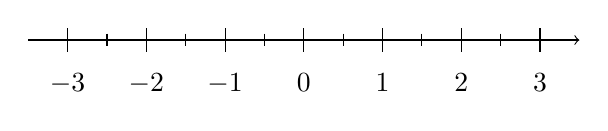
\begin{tikzpicture}[scale=1]
            \draw[->] (-3.5,0) -- (3.5,0);
            \foreach \i in {-3,...,3} {
                \draw (\i,0.15) -- (\i,-0.15);
                \node[below] at (\i,-0.3) {$\i$};
            }
            \foreach \i in {-2.5,-1.5,-0.5,0.5,1.5,2.5} {
                \draw (\i,0.08) -- (\i,-0.08);
            }
        \end{tikzpicture}
    \end{center}
\end{exercise}
 
\newpage
\section{Exercices mélangés}
\setcounter{exercise}{0}

\begin{exercise}
Rends les fractions suivantes irréductibles. Écris les différentes étapes lorsque cela est nécessaire.

\begin{enumerate}[cols=3]
\item $\dfrac{12}{18}=$
\item $\dfrac{16}{24}=$
\item $\dfrac{28}{42}=$
\item $\dfrac{45}{60}=$
\item $\dfrac{54}{72}=$
\item $\dfrac{30}{45}=$
\item $\dfrac{36}{48}=$
\item $\dfrac{49}{63}=$
\item $\dfrac{81}{108}=$
\item $\dfrac{64}{96}=$
\end{enumerate}
\end{exercise}

\begin{exercise}
Calcule puis simplifie le résultat lorsque c'est possible.

\begin{enumerate}[cols=3]
\item $\dfrac{3}{8}+\dfrac{2}{8}=$
\item $\dfrac{7}{9}+\dfrac{1}{9}=$
\item $\dfrac{5}{12}+\dfrac{4}{12}=$
\item $\dfrac{11}{15}+\dfrac{2}{15}=$
\item $\dfrac{6}{7}+\dfrac{1}{7}=$
\item $\dfrac{14}{20}+\dfrac{5}{20}=$
\item $\dfrac{8}{13}+\dfrac{3}{13}=$
\item $\dfrac{9}{10}+\dfrac{1}{10}=$
\item $\dfrac{7}{18}+\dfrac{5}{18}=$
\item $\dfrac{13}{24}+\dfrac{7}{24}=$
\item $\dfrac{7}{8}-\dfrac{3}{8}=$
\item $\dfrac{11}{12}-\dfrac{5}{12}=$
\item $\dfrac{15}{20}-\dfrac{7}{20}=$
\item $\dfrac{16}{25}-\dfrac{9}{25}=$
\item $\dfrac{17}{18}-\dfrac{8}{18}=$
\item $\dfrac{19}{30}-\dfrac{4}{30}=$
\item $\dfrac{12}{14}-\dfrac{5}{14}=$
\item $\dfrac{23}{40}-\dfrac{11}{40}=$
\item $\dfrac{29}{36}-\dfrac{17}{36}=$
\item $\dfrac{21}{28}-\dfrac{9}{28}=$
\end{enumerate}
\end{exercise}

\newpage
\begin{exercise}
Pour chaque droite graduée :
\begin{itemize}
\item écris la fraction correspondant à la lettre.
\item place ensuite la fraction demandée sur la droite.
\end{itemize}

\begin{enumerate}[itemsep=1cm]

%-------------------------
\item
\begin{center}
\begin{tikzpicture}[scale=1]
\draw[->](-0.3,0)--(4.3,0);
\foreach \x in {0,...,4}{\draw(\x,0.12)--(\x,-0.12);}
\node[below] at (0,-0.2){$0$};
\node[below] at (4,-0.2){$1$};
\fill (3,0) circle(2pt) node[above]{$A$};
\end{tikzpicture}
\end{center}

$A=$\dotfill \hfill Place $\dfrac14$

%-------------------------
\item
\begin{center}
\begin{tikzpicture}[scale=0.8]
\draw[->](-0.3,0)--(5.3,0);
\foreach \x in {0,...,5}{\draw(\x,0.12)--(\x,-0.12);}
\node[below] at (0,-0.2){$0$};
\node[below] at (5,-0.2){$1$};
\fill (2,0) circle(2pt) node[above]{$B$};
\end{tikzpicture}
\end{center}

$B=$\dotfill \hfill Place $\dfrac45$

%-------------------------
\item
\begin{center}
\begin{tikzpicture}[scale=0.7]
\draw[->](-0.3,0)--(6.3,0);
\foreach \x in {0,...,6}{\draw(\x,0.12)--(\x,-0.12);}
\node[below] at (0,-0.2){$0$};
\node[below] at (6,-0.2){$1$};
\fill (5,0) circle(2pt) node[above]{$C$};
\end{tikzpicture}
\end{center}

$C=$\dotfill \hfill Place $\dfrac13$

%-------------------------
\item
\begin{center}
\begin{tikzpicture}[scale=0.7]
\draw[->](-0.3,0)--(8.3,0);
\foreach \x in {0,...,8}{\draw(\x,0.12)--(\x,-0.12);}
\node[below] at (0,-0.2){$0$};
\node[below] at (8,-0.2){$1$};
\fill (6,0) circle(2pt) node[above]{$D$};
\end{tikzpicture}
\end{center}

$D=$\dotfill \hfill Place $\dfrac18$

%-------------------------
\item
\begin{center}
\begin{tikzpicture}[scale=0.6]
\draw[->](-0.3,0)--(10.3,0);
\foreach \x in {0,...,10}{\draw(\x,0.12)--(\x,-0.12);}
\node[below] at (0,-0.2){$0$};
\node[below] at (10,-0.2){$1$};
\fill (7,0) circle(2pt) node[above]{$E$};
\end{tikzpicture}
\end{center}

$E=$\dotfill \hfill Place $\dfrac9{10}$

%-------------------------
\item
\begin{center}
\begin{tikzpicture}[scale=0.6]
\draw[->](-0.3,0)--(12.3,0);
\foreach \x in {0,...,12}{\draw(\x,0.12)--(\x,-0.12);}
\node[below] at (0,-0.2){$0$};
\node[below] at (12,-0.2){$1$};
\fill (4,0) circle(2pt) node[above]{$F$};
\end{tikzpicture}
\end{center}

$F=$\dotfill \hfill Place $\dfrac{11}{12}$

%-------------------------
\item
\begin{center}
\begin{tikzpicture}[scale=0.8]
\draw[->](-0.3,0)--(8.3,0);
\foreach \x in {0,...,8}{\draw(\x,0.12)--(\x,-0.12);}
\node[below] at (0,-0.2){$0$};
\node[below] at (4,-0.2){$\frac12$};
\node[below] at (8,-0.2){$1$};
\fill (5,0) circle(2pt) node[above]{$G$};
\end{tikzpicture}
\end{center}

$G=$\dotfill \hfill Place $\dfrac38$

%-------------------------
\item
\begin{center}
\begin{tikzpicture}[scale=0.8]
\draw[->](-0.3,0)--(10.3,0);
\foreach \x in {0,...,10}{\draw(\x,0.12)--(\x,-0.12);}
\node[below] at (0,-0.2){$0$};
\node[below] at (5,-0.2){$\frac12$};
\node[below] at (10,-0.2){$1$};
\fill (8,0) circle(2pt) node[above]{$H$};
\end{tikzpicture}
\end{center}

$H=$\dotfill \hfill Place $\dfrac25$

%-------------------------
\item
\begin{center}
\begin{tikzpicture}[scale=0.6]
\draw[->](-0.3,0)--(16.3,0);
\foreach \x in {0,...,16}{\draw(\x,0.12)--(\x,-0.12);}
\node[below] at (0,-0.2){$0$};
\node[below] at (8,-0.2){$\frac12$};
\node[below] at (16,-0.2){$1$};
\fill (11,0) circle(2pt) node[above]{$I$};
\end{tikzpicture}
\end{center}

$I=$\dotfill \hfill Place $\dfrac{15}{16}$

%-------------------------
\item
\begin{center}
\begin{tikzpicture}[scale=0.5]
\draw[->](-0.3,0)--(20.3,0);
\foreach \x in {0,...,20}{\draw(\x,0.12)--(\x,-0.12);}
\node[below] at (0,-0.2){$0$};
\node[below] at (10,-0.2){$\frac12$};
\node[below] at (20,-0.2){$1$};
\fill (17,0) circle(2pt) node[above]{$J$};
\end{tikzpicture}
\end{center}

$J=$\dotfill \hfill Place $\dfrac7{20}$

\end{enumerate}
\end{exercise}

\begin{exercise}
Place les fractions suivantes sur les droites graduées.

\begin{enumerate}

%----------------------------
\item Place les fractions :
\[
-\frac32,\qquad -\frac12,\qquad \frac34,\qquad \frac74
\]

\begin{center}
\begin{tikzpicture}[x=3cm,y=1cm]
\draw[->] (-2.2,0)--(2.2,0);

\foreach \x in {-2,-1.75,...,2}{
    \draw (\x,0.12)--(\x,-0.12);
}

\node[below] at (-2,-0.15){$-2$};
\node[below] at (-1,-0.15){$-1$};
\node[below] at (0,-0.15){$0$};
\node[below] at (1,-0.15){$1$};
\node[below] at (2,-0.15){$2$};
\end{tikzpicture}
\end{center}

%----------------------------
\item Place les fractions :
\[
-\frac85,\qquad -\frac35,\qquad \frac75,\qquad \frac95
\]

\begin{center}
\begin{tikzpicture}[x=3cm,y=1cm]
\draw[->] (-2.2,0)--(2.2,0);

\foreach \x in {-2,-1.8,...,2}{
    \draw (\x,0.12)--(\x,-0.12);
}

\node[below] at (-2,-0.15){$-2$};
\node[below] at (-1,-0.15){$-1$};
\node[below] at (0,-0.15){$0$};
\node[below] at (1,-0.15){$1$};
\node[below] at (2,-0.15){$2$};
\end{tikzpicture}
\end{center}

%----------------------------
\item Place les fractions :
\[
-\frac{13}{8},\qquad -\frac38,\qquad \frac98,\qquad \frac{15}{8}
\]

\begin{center}
\begin{tikzpicture}[x=3cm,y=1cm]
\draw[->] (-2.2,0)--(2.2,0);

\foreach \x in {-2,-1.875,...,2}{
    \draw (\x,0.10)--(\x,-0.10);
}

\node[below] at (-2,-0.15){$-2$};
\node[below] at (-1,-0.15){$-1$};
\node[below] at (0,-0.15){$0$};
\node[below] at (1,-0.15){$1$};
\node[below] at (2,-0.15){$2$};
\end{tikzpicture}
\end{center}

%----------------------------
\item Place les fractions :
\[
-\frac74,\qquad -\frac14,\qquad \frac54,\qquad \frac32
\]

\begin{center}
\begin{tikzpicture}[x=3cm,y=1cm]
\draw[->] (-2.2,0)--(2.2,0);

\foreach \x in {-2,-1.75,...,2}{
    \draw (\x,0.12)--(\x,-0.12);
}

\node[below] at (-2,-0.15){$-2$};
\node[below] at (-1,-0.15){$-1$};
\node[below] at (0,-0.15){$0$};
\node[below] at (1,-0.15){$1$};
\node[below] at (2,-0.15){$2$};
\end{tikzpicture}
\end{center}

\end{enumerate}

\end{exercise}

\begin{exercise}
     Sarah dit : « J'ai bu les $\frac{3}{10}$ d'une bouteille de jus d'orange de un litre le matin, et j'en ai bu encore $\frac{4}{10}$ durant l'après-midi. »
    \begin{enumerate}
        \item Quelle fraction totale de la bouteille Sarah a-t-elle bue durant la journée ?
        \item Quelle fraction de jus reste-t-il dans la bouteille ?
    \end{enumerate}
\end{exercise}
 
\begin{exercise}
     Bruno récolte les pommes de son verger. Il en vend immédiatement le quart ($\frac{1}{4}$) à ses voisins. Après cette vente, il lui reste exactement $15$ kg de pommes pour faire des tartes.
 
    Quelle était la masse totale (en kg) de sa récolte de pommes au départ ? (Aide-toi d'un schéma d'une boîte coupée en parts égales si nécessaire !)
\end{exercise}
 
\begin{exercise}
    Un tiers ($\frac{1}{3}$) d'un grand vase est rempli d'eau. On ajoute ensuite une quantité d'eau égale aux deux tiers ($\frac{2}{3}$) du volume libre restant.
 
    Au total, quelle part (fraction) du volume global du vase est maintenant remplie d'eau ? Explique ton raisonnement par un calcul ou un graphique complet.
\end{exercise}
 
\begin{exercise}
    Si tu as bien compris comment simplifier des nombres, tente de simplifier ces expressions avec des lettres (où $a$, $b$ et $c$ sont des nombres entiers non nuls).
    \begin{enumerate}[cols=1, itemsep=1.5cm]
        \item $\dfrac{3 \cdot b}{7 \cdot b} = $
        \item $\dfrac{16 \cdot a}{8 \cdot a} = $
        \item $\dfrac{a \cdot b \cdot c}{a \cdot b \cdot d} = $
    \end{enumerate}
\end{exercise}

\newpage
\section*{Mots-clès}
\begin{enumerate}[cols=2, label=\textbf{\arabic*.}]
    \item Fraction
    \item Numérateur
    \item Dénominateur
    \item Division
    \item Simplification
    \item Réduire
    \item Droite graduée
    \item Inverse
\end{enumerate}

\section*{Attendus}
\begin{enumerate}[label=\textbf{\arabic*.}]
    \item Additionner deux fractions d’une même grandeur.
    \item Placer sur la droite graduée des nombres décimaux positifs et leurs opposés.
    \item Identifier un nombre naturel, un nombre entier, un nombre rationnel positif ou négatif (écrit sous la forme fractionnaire, décimale).
    \item Associer la fraction nombre à un quotient ($69 : 4 = \frac{69}{4}$).
    \item Associer différentes écritures d’un même nombre : décimale, fractionnaire, pourcentage.
    \item Associer l’expression « inverse d’un nombre » à son écriture mathématique. Ex. : l'inverse de $2$ est $\frac{1}{2}$.
    \item Expliquer les notions de valeur exacte, de valeurs approchées (par excès et par défaut) et d’arrondi.
    \item Interpréter l’écriture décimale fournie par un outil numérique.
    \item Transformer l’écriture d’un nombre en une écriture équivalente (écriture fractionnaire et écriture décimale).
    \item Écrire une fraction équivalente à une autre.
    \item Simplifier une fraction.
    \item Rendre une fraction irréductible.
    \item Placer un nombre (naturel, entier, rationnel positif ou négatif) sur une droite graduée.
    \item Comparer deux nombres (entiers, rationnels) en utilisant le symbole adéquat ( <, >, = ).
    \item Encadrer un nombre entier, un nombre rationnel à l’unité, au dixième ou au centième près.
    \item Ordonner des nombres entiers, des nombres rationnels sous forme décimale et/ou fractionnaire, par ordre croissant ou décroissant.
    \item Déterminer la valeur approchée d’un nombre rationnel par défaut ou par excès, le degré de précision étant donné.
    \item Associer à l’addition et à la soustraction de deux nombres entiers ou décimaux (positifs ou négatifs) un déplacement ou écart sur la droite numérique.
    \item Calculer (nombres entiers et décimaux) en utilisant les propriétés des opérations (commutativité, associativité, neutre, absorbant) et la distributivité.
    \item Calculer (nombres entiers et décimaux) en utilisant les priorités des opérations.
    \item Utiliser la calculatrice pour vérifier le résultat d’une opération (nombres entiers et nombres décimaux).
\end{enumerate}

\end{document}